\section{System/Subsystem Design Description}

\subsection{System wide design decisions}
In dit hoofdstuk worden, zoals de tital al verraad, de design decisions behandeld. Hieronder vallen bijvoorbeeld
input/outputs van het systeem, gedrag keuzes en andere onderdelen die voor het gehele systeem gelden


\subsubsection{Camera}
De camera zal dienen als de zintuigen van de drones. Echte bijen gebruiken reuk en zicht om hun eten op te sporen. Dat betekent dat het vanzelfsprekend is om hiervoor een camera te gebruiken, gezien dit zicht vervangt. De hersenen van elk levend wezen is zo ingesteld om onderscheid te kunnen maken tussen verschillende objecten die wij middels zicht kunnen observeren. Dit onderscheid zal ook gemaakt moeten worden binnen de simulatie, gezien dit informatie is die een bij aanstuurt om een bepaalde gedrag te vertonen.

\subsubsection{Server}
Omdat het een gecentraliseerd systeem is worden de meeste acties bepaald door een centraal subsysteem, in dit geval is dat de server.
Vanuit de server worden de drones aantgestuurd en wordt informatie van en naar de simulatie en camera verstuurd. Voor alle communicatie
wordt een MQTT broker gebruikt.

\subsubsection*{Gedrag}
Met gedrag worden de keuzes bedoelt die het systeem maakt, hiermee worden de basis van het systeem bepaald.
\begin{enumerate}
    \item Bij opstart word een drone naar de voedsel bron gestuurd.
    \item Wanneer de drone deze locatie heeft berijkt zal hij trugkeren naar eht startpunt
    \item De Drone danst om de locatie te delen met de andere drones
    \item Meerdere drones worden gestuurd om het voedsel op te halen
    \item Wanneer het laatste voedsel uit de bron is gehaald en alle drones binnen zijn worden een nieuwe scout gestruurd
\end{enumerate}

\subsubsection*{Inputs/outputs}
De server krijgt vanuit meerdere punten informatie binnen en verstuurd het ook naar meerdere subsystemen.
Deze inputs en outputs worden uitgebreided in het hoofdstuk Interface Design Decisions.


\begin{description}
    \item[Input] Camera informatie
    \item[Input] Simulatie informatie
    \item[Output] Drone gedrag
    \item[Output] Simulatie informatie
\end{description}

\subsubsection{Simulatie}
De simulatie is een eenvoudig manier om een overzicht te krijgen over het gehele project. Dit komt omdat het net als met de echte server en drone, samenhangt met de rest van het geheel. Zo neemt de simulatie als input de coordinaten van de drones. Net als de echte server verwerkt de simulatie de coordinaten om uiteindelijk als output signalen door te geven aan de gesimuleerde drones. Deze signalen zijn de commandos die de drones uit moeten voeren. Dit gebeurt allemaal op een hoge snelheid gezien de simulatie op een sterke Windows laptop afgebeeld wordt. De limiet hieraan is dus de snelheid van de ingekomen locatie data. Om deze data veilig te ontvangen wordt er een MQTT server gebruikt die vergrendeld is met inloggegevens. Gezien de simulatie zelf lokaal op een PC is, zijn hier verder geen beveiligingsrisicos aan gekoppeld. Omdat het een simulatie is, wordt er een groot belang gehecht aan toegankelijkheid van data. De beste, en soms wel enige, manier om een simulatie te testen is door gebruik te maken van verschillende variabelen en states waar een simulatie zich in kan bevinden. Zo kan een simulatie gebruikt worden om een zo realistisch mogelijk gesimuleerde omgeving weer te geven.


\subsection{System architectural design}

\subsubsection{System components}
Hier wordt een opsomming gegeven van alle hardware en software componenten gegeven, 

\begin{description}
    \item[Software] Camera
    \item[Software] MQTT Broker
    \item[Software] simulatie
    \item[Software] Server
    \item[Hardware] Picam
    \item[Hardware] Crazyflie
\end{description}

\subsubsection{System architecture}
Diagram met hardware en software componenten van het gehelen systeem en de relatie tussen deze onderdelen
\subsubsection*{Camera}
Aangezien het project inhoudt dat een aantal bijen gesimuleerd wordt, is het nodig om hun zintuigen ook te simuleren. Dit gebeurt door middel van een camera aan een raspberry pi. Hier zullen uiteraard eisen aan zitten, maar zullen in de SRS vermeldt worden. Om deze camera draadloos te laten werken is er ook een batterij pack nodig.

\subsubsection*{Server}
Hieronder is de relatie te zien tussen de verschillende onderedelen van de Server. Hierin zijn ook de componenten meegenomen waar de Server mee communiceerd buiten zichzelf. Op deze manier is een overview van het volledige systeem weergegeven.
De eerste communicatie begint wanneer de Camera begint met communiceren naar de MQTT broker.
\begin{center}
    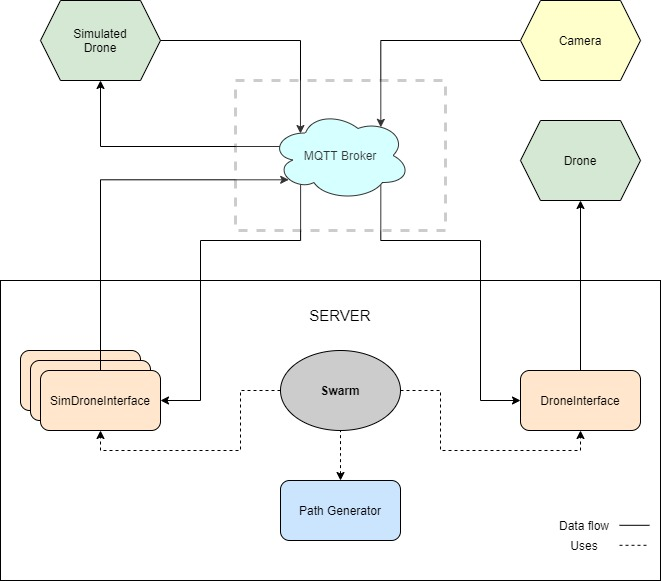
\includegraphics[scale=0.5]{../IMAGES/ServerV3.jpg}
\end{center}



\subsubsection*{Simulatie}
    \begin{center}
    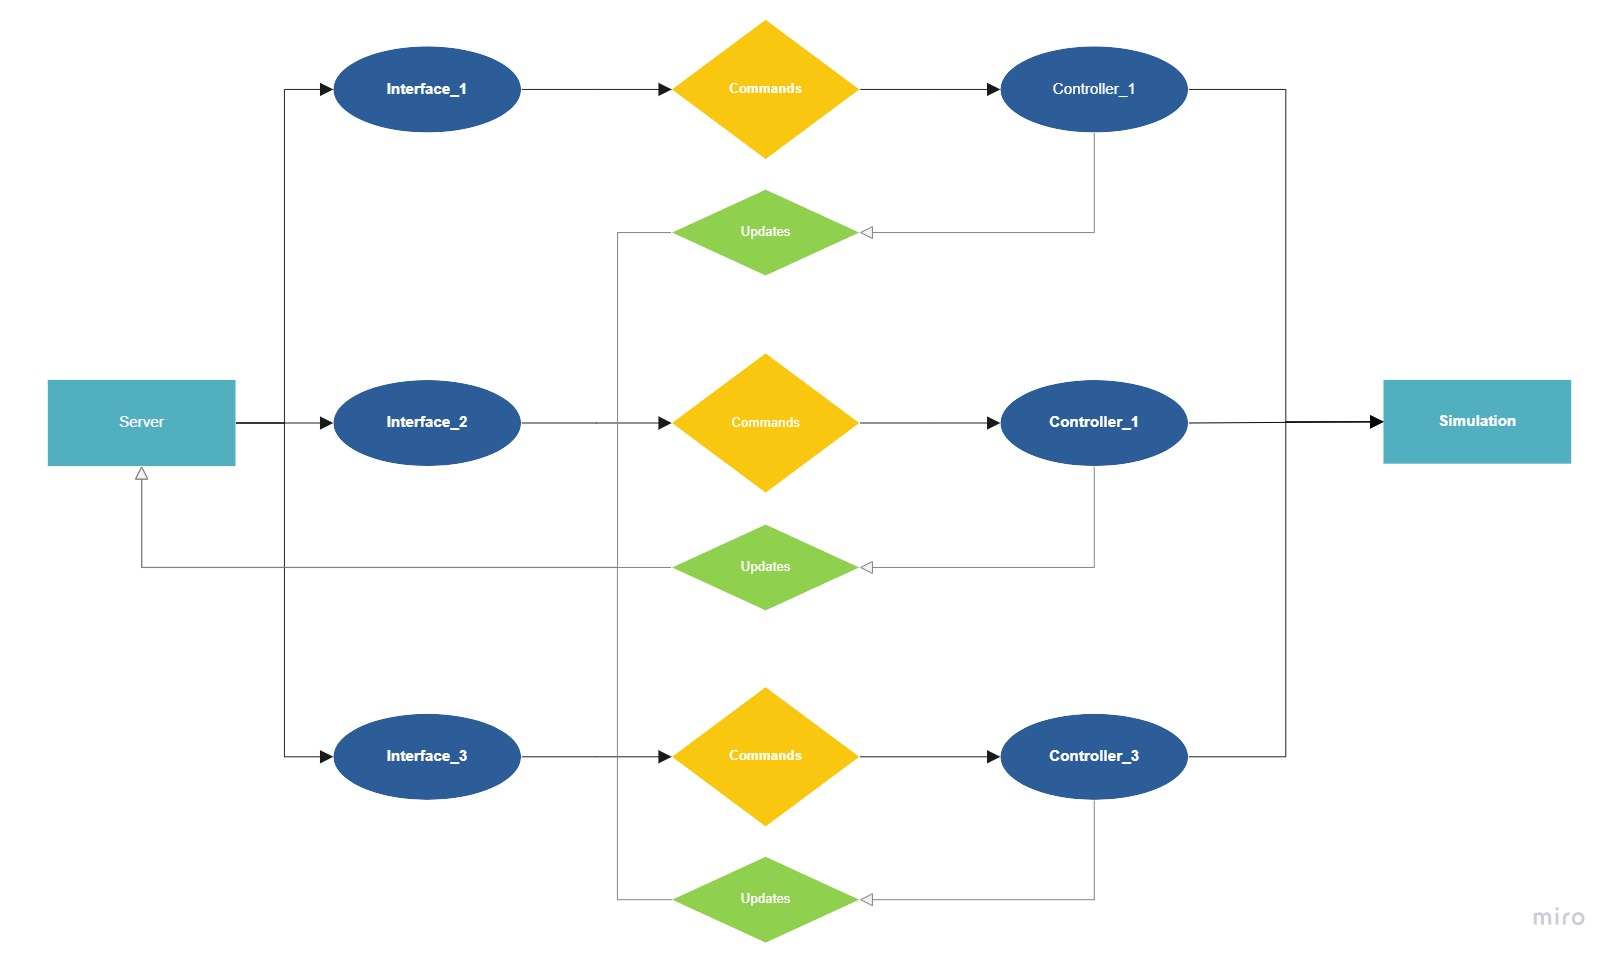
\includegraphics[scale=0.22]{../IMAGES/Simulation Interaction.jpg}
    \end{center}
    Het diagram hierboven weergeeft de communicatie tussen de simulatie en de server. In de simulatie
    wordt het gedrag van bijen met behulp van 3 ontworpen drones gesimuleerd. Om dat mogelijk te maken
    zijn voor de input en de output de volgende ontwerp keuzes gemaakt: \\

    \begin{description}\setlength{\itemindent}{0.1cm}
        \item[INPUT:] \hfill
        \begin{enumerate}
            \item De input voor de simulatie is altijd een opdracht naar een controller. Deze opdracht is een
            actie die een drone moet uitvoeren waarbij een positie meegegeven wordt  naarr de volgende verplaatsingsstap.
            Dit wordt mogelijk gemaakt door te communiceren tegen een opgebouwde interface. Deze
            interface communiceerd dan vervolgens tegen een controller die een gesimuleerde drone bestuurd.
        \end{enumerate}
        
        \item[OUTPUT:] \hfill
        \begin{enumerate}
            \item De output bij deze simulatie is verplaatsing van de gesimuleerde drone naar een geplannde positie.
            \item Daarnaast is er ook een andere continue output van de simulatie. Dat is een bericht die afkomstig
            is van een controller. Een controller stuurt om de bepaalde tijd een bericht naar de server met
            de informatie over de positie van de bestuurde drone.
        \end{enumerate}


    \end{description}

    \newpage
\subsection{System architectural design}
Uiteraard is het project een samenhangend geheel. Dit betekent dat er onderdelen zijn die afhankelijk zijn van andere onderdelen. Deze onderdelen zullen vermeld worden.

\subsubsection*{System components}
De relatie tussen deze onderdelen is te zien de paragraaf architecture onder het kopje server. In deze afbeelding is te zien hoe zowel de harware als software in relatie staat met elkaar.
